% mainfile: ../../main.tex
\chapter{Observations}\label{ch:exp:observations}
\AutoLettrine{Pidgeons}
\section{Transfer-matrix method simulations of the membrane structure}\label{sec:exp:tmm}
The \gls{tmm} is a computationally efficient method of obtaining the electric field in layered structures.
In this section, I perform simulations of the heterostructure membranes investigated in \thispart using the \pymoosh package~\cite{Langevin2024} to elucidate the observed quenching of \gls{pl} when illuminating gate electrodes as well as the overall optical efficiency.\sidenote{
    Strictly speaking, the term \acrshort{tmm} only refers to one of the several formalisms implemented in the \pymoosh package.
    While fast, it is not the most numerically stable, and other methods may be preferred if wall time is not a limiting issue.
}
I will first briefly recap the simulation method following \citer{Langevin2024}.
For more details, refer to \ibid and references therein.

Consider a layered structure along $z$ with interfaces at $z_i, i\in\lbrace 0, 1, \dotsc, N+1\rbrace$ that is translationally invariant along $x$ and $y$.
Each layer $i$ may consist of a different dielectric material characterized by a (complex) relative permittivity $\epsilon_{r,i}$.\sidenote{
    We disregard magnetic materials with relative permeability $\mu_r\neq 1$ for simplicity.
}
The electric field component along $y$ of an electromagnetic wave \gls{te} mode originating in some far away point satisfies the Helmholtz equation
\begin{equation}\label{eq:exp:tmm:helmholtz}
    \pdv[2]{E_y}{z} + \gamma_i^2 E_y = 0,
\end{equation}
where $\gamma_i = \sqrt{\epsilon_{r,i}k_0^2 - k_x^2}$ with $k_0=\flatfrac{\omega}{c}$ the wave vector in vacuum and $k_x$ the component along $x$.
In layer $i$ of the structure, the solution to \cref{eq:exp:tmm:helmholtz} may be written as a superposition of plane waves incident and reflected on the lower and upper interfaces~\cite{Langevin2024},
\begin{equation}\label{eq:exp:tmm:fields}
    \begin{dcases}
        E_{y,i}(z) = A_i^{+}\exp{\i\gamma_i[z-z_{i}]} + B_i^{+}\exp{-\i\gamma_i[z-z_{i}]}, \\
        E_{y,i}(z) = A_i^{-}\exp{\i\gamma_i[z-z_{i+1}]} + B_i^{-}\exp{-\i\gamma_i[z-z_{i+1}]},
    \end{dcases}
\end{equation}
where the coefficients with superscript $+$ ($-$) are referenced to the phase at the upper (lower) interface, respectively.
Matching these solutions at $z=z_i$ for all $i$ to satisfy the interface conditions imposed by Maxwell's equations gives rise to a linear system of equations, the solution to which can be obtained through several different methods.

A particularly simple method is the \acrlong{tmm} ($T$-matrix formalism), which corresponds to writing the interface conditions at $z=z_i$ as the matrix equation
\begin{equation}\label{eq:exp:tmm:interface}
    \pmqty{A_{i+1}^{+}\\B_{i+1}^{+}} = T_{i,i+1}\pmqty{A_{i}^{-}\\B_{i}^{-}}
\end{equation}
with
\begin{equation}\label{eq:exp:tmm:T}
    T_{i,i+1} = \frac{1}{2\gamma_{i+1}}\begin{pmatrix}
        \gamma_{i} + \gamma_{i+1} & \gamma_{i} - \gamma_{i+1} \\
        \gamma_{i} - \gamma_{i+1} & \gamma_{i} + \gamma_{i+1}
    \end{pmatrix}
\end{equation}
the transfer matrix for interface $i$.
Connecting the coefficients for adjacent interfaces within a layer of height $h_i = z_{i+1} - z_{i}$ requires propagating the phase,
\begin{equation}\label{eq:exp:tmm:propagation}
    \pmqty{A_{i}^{-}\\B_{i}^{-}} = C_{i}\pmqty{A_{i}^{+}\\B_{i}^{+}},
\end{equation}
with
\begin{equation}\label{eq:exp:tmm:C}
    C_{i} = \exp\left\lbrace\diag(-\i\gamma_i h_i, \i\gamma_i h_i)\right\rbrace.
\end{equation}
Iterating \cref{eq:exp:tmm:C,eq:exp:tmm:T}, the total transfer matrix $T = T_{0,N+1}$ then reduces to the matrix product
\begin{equation}\label{eq:exp:tmm:T:total}
    T = T_{N,N+1}\prod_{i=0}^{N-1} T_{i,i+1} C_i.
\end{equation}
From $T$, the reflection and transmission coefficients can be obtained as $r=A_0^{-}=-\flatfrac{T_{01}}{T_{00}}$ and $t=B_{N+1}^{+}=rT_{10} + T_{11}$.
Taking the absolute value square of reflection and transmission coefficients then yields the reflectance \reflectance and the transmittance \transmittance, which correspond to the fraction of total incident power being reflected and transmitted, respectively.
To obtain the absorptance \absorptance, the fraction of power being absorbed, in layer $i$, one can compute the difference of the $z$-components of the Poynting vectors (\cf \cref{eq:setup:optics:coupling:poynting}) at the top of layers $i$ and $i+1$.
In the \gls{te} case considered here, \cref{eq:setup:optics:coupling:poynting} reduces to~\cite{Langevin2024}
\begin{equation}\label{eq:exp:tmm:poynting}
    \bvec{S}_i = \re\left[\frac{\gamma_i^{\ast}}{\gamma_0}\left(A_i^{+} - B_i^{+}\right)^{\ast}\left(A_i^{+} + B_i^{+}\right)\right]
\end{equation}
and is hence straightforward to extract from the calculation of either the $S$ or $T$ matrices.

\Cref{eq:exp:tmm:T:total} is simple to evaluate on a computer, making this method attractive for numerical applications.
However, the opposite signs in the argument of the exponentials in \cref{eq:exp:tmm:C} can lead to instabilities for evanescent waves ($\gamma_i\in\mathbb{C}$) due to finite-precision floating point arithmetic~\cite{Duetz}.
Rewriting \cref{eq:exp:tmm:T} to have incoming and outgoing fields on opposite sides of the equality alleviates this issue while sacrificing the simple matrix-multiplication composition rule in what is known as the scattering matrix ($S$-matrix) formalism.
Finally, note that for a thorough accounting of in- and out-going field amplitudes, excitonic effects should be included, for example using the approach by \citet{DAndrea1990}.

Beyond the calculation of the aforementioned coefficients, the \gls{tmm} formalism also allows to compute the full spatial dependence of the fields.
Two cases are implemented in \pymoosh: irradiation of the layered structured with a Gaussian beam rather than plane waves of infinite extent, and a current line source inside the structure.
In the first case, the previously assumed translational invariance along $x$ leading to a plane-wave spatial dependence is replaced by a superposition of plane waves weighted with a normally distributed amplitude,\sidenote{
    \Ie, the inverse Fourier transform of $\mc{E}_0(k_x) E_{y,i}(k_x, z)$.
}
\begin{equation}\label{eq:exp:tmm:gauss:x}
    E_{y,i}(x,z) = \exp(\i k_x x)\rightarrow \int\ddf{k_x}\mc{E}_0(k_x) E_{y,i}(k_x, z)\exp(\i k_x x),
\end{equation}
with (\cf \cref{eq:setup:gaussian})
\begin{equation}\label{eq:exp:tmm:gauss:ampl}
    \mc{E}_0(k_x) = \frac{w_0}{2\sqrt{\pi}}\exp\left\lbrace - \i k_x x_0 -\left[\frac{w_0 k_x}{2}\right]^2\right\rbrace
\end{equation}
and
\begin{equation}\label{eq:exp:tmm:gauss:z}
    E_{y,i}(k_x, z) = A_{i}^{-}\exp\lbrace\i\gamma_i(k_x)[z-z_{i+1}]\rbrace + B_{i}^{+}\exp\lbrace -\i\gamma_i(k_x)[z-z_{i}]\rbrace,
\end{equation}
and where we considered only normal incidence for simplicity.

In the second case, \citet{Langevin2024} consider an AC current $I$ flowing through a translationally invariant, one-dimensional wire along $y$ at $x=x_{\mr{s}}$.
This introduces a source term into the Helmholtz equation, \cref{eq:exp:tmm:helmholtz}, which, upon Fourier transforming in $x$ direction, leads to
\begin{equation}\label{eq:exp:tmm:helmholtz:green}
    \pdv[2]{\hat{E}_y}{z} + \gamma_i^2\hat{E}_y = -\i\omega\mu_0 I\delta(z)\exp(\i k_x x_{\mr{s}}).
\end{equation}
The electric field $\hat{E}_{y,i}(k_x, z)$ is thus proportional to the Green's function of \cref{eq:exp:tmm:helmholtz:green} and can be obtained using a similar procedure as in the case of a distant source incident on the structure by matching the interface conditions.
Performing the inverse Fourier transform by means of \cref{eq:exp:tmm:gauss:x} with constant weights, $\mc{E}_0(k_x)\equiv 1$, then yields the two-dimensional spatial distribution of the electric field, $E_{y,i}(x, z)$.

\begin{figure}
    \centering
    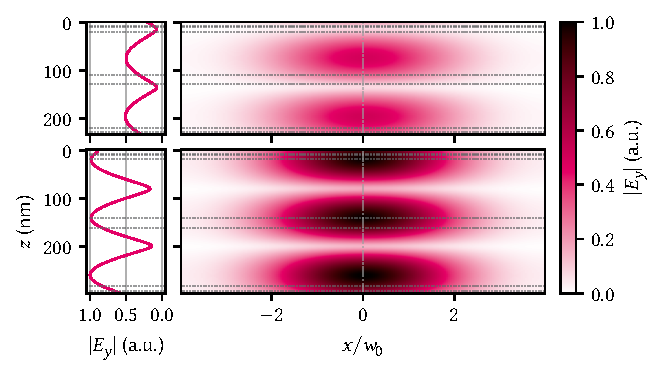
\includegraphics{img/pdf/experiment/tmm_field}
    \caption[\imgsource{img/py/experiment/tmm.py}]{
        Absolute value of the electric field inside the double-gated heterostructure under illumination with a Gaussian beam at $\lambda=\qty{825}{\nano\meter}$ from the top.
        Top (bottom) panels show the structure with the default (optimized) barrier thickness of \qty{90}{\nano\meter} (\qty{122}{\nano\meter}), respectively.
        Dotted horizontal lines indicate interfaces between different materials while the vertical dash-dotted line indicates the position of the line cuts shown in the left column.
        Increasing the thickness of the barrier has two beneficial effects; first, the overall field intensity inside the structure is higher by a factor of two, and second, there is a peak rather than a knot in the \gls{qw} at a depth of $\sim\qty{120}{\nano\meter}$ ($\sim\qty{150}{\nano\meter}$), leading to enhanced absorption.
    }
    \label{fig:exp:tmm:field}
\end{figure}

\begin{margintable}
    \centering
    \footnotesize
    \caption{
        Absorptance $\mathscr{A}$ and reflectance $\mathscr{R}$ in the \gls{qw} for different configurations of the heterostructure.
        \enquote{Bare} is the standard structure without gate electrodes.
        \enquote{TG} and \enquote{BG} are with a gate on either the top or bottom side.
        \enquote{TG+BG} is with gates on both sides as on a trap site.
    }
    \label{tab:exp:tmm:absorptance_reflectance}
    % This table is automatically generated by img/py/experiment/tmm.py
\begin{tabular}{lSS}
\toprule
 & {$\mathscr{A}$ (\unit{\percent})} & {$\mathscr{R}$ (\unit{\percent})} \\
\midrule
Bare & 2.9 & 22.4 \\
TG & 1.8 & 42.0 \\
BG & 0.5 & 82.7 \\
TG+BG & 0.4 & 84.8 \\
\bottomrule
\end{tabular}

\end{margintable}

\begin{marginfigure}
    \centering
    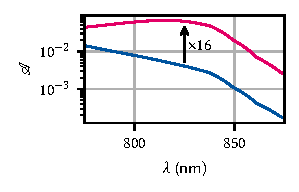
\includegraphics{img/pdf/experiment/tmm_absorptance}
    \caption[\imgsource{img/py/experiment/tmm.py}]{
        \Gls{qw} absorptance \absorptance in a heterostructure with default (blue) and optimized (magenta) barrier thickness and top and bottom gates as function of wavelength.
        Optimization was performed at \qty{825}{\nano\meter} using the differential evolution algorithm implemented in \pymoosh, resulting in a barrier thickness of \qty{122}{\nano\meter} and an absorptance better by a factor of \num{16} at \qty{6.3}{\percent}.
    }
    \label{fig:exp:tmm:wavelengths}
\end{marginfigure}
\clearpage
\begin{marginfigure}
    \centering
    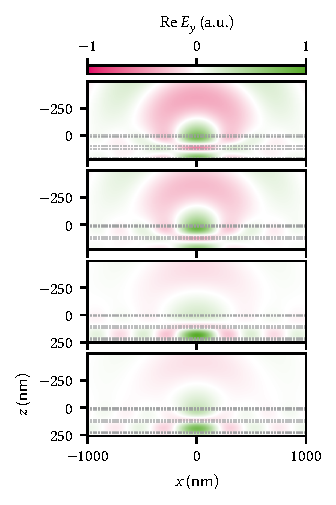
\includegraphics{img/pdf/experiment/tmm_green}
    \caption[\imgsource{img/py/experiment/tmm.py}]{
        Real part of the electric field emitted by a current line located in the \gls{qw} (black point) for different cases of the unoptimized structure.
        From top to bottom: bare heterostructure, top gate, bottom gate, top and bottom gate.
        The half space $z<0$ is the air above the membrane in the direction of the objective lens and the dotted lines indicate interfaces between materials.
        Evidently, the bottom gate reduces the amplitude in the upper half of the membrane and thereby the outcoupling efficiency compared to the structures with just a top gate, consistent with what is observed in the experiment.
    }
    \label{fig:exp:tmm:green}
\end{marginfigure}

\begin{marginfigure}
    \centering
    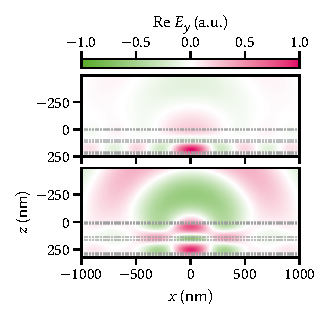
\includegraphics{img/pdf/experiment/tmm_green_opt_tgbg}
    \caption[\imgsource{img/py/experiment/tmm.py}]{
        Real part of the electric field emitted by a current line located in the \gls{qw} (black point) for the default (top) and optimized (bottom) structures with top and bottom gates.
        Optimizing the barrier thickness for absorption in the \gls{qw} evidently also drastically improves the outcoupling efficiency into the halfspace $z<0$.
    }
    \label{fig:exp:tmm:green:opt:tgbg}
\end{marginfigure}
\clearpage

\begin{marginfigure}
    \centering
    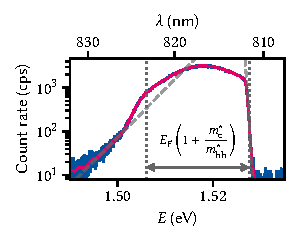
\includegraphics{img/pdf/experiment/2deg_pl}
    \caption[
        \sampleid{Doped M1_05_49-2}
        \thewavelength{795}.
        \thepower{0.92}{\micro}
        \protect\newline
        \imgsource{img/py/experiment/pl.py}
    ]{
        \Gls{pl} of the bare \gls{2deg}.
        Magenta line is a smoothing spline fit to the data.
        Indicated by dotted gray lines are the Fermi edge at high and the band edge at low energy.
        The Fermi edge has a Fermi distribution (exponential indicated by a dashed gray line) whose temperature is typically much higher than the lattice temperature ($\sim\qty{1}{\kelvin}$).
        Below the band edge there is an exponential tail (dashed gray line) due to impurities that permeates far into the gap.
    }
    \label{fig:exp:pl:2deg}
\end{marginfigure}

\Cref{fig:exp:pl:2deg} shows a typical \gls{pl} spectrum obtained on the bare, unbiased \gls{qw} of a doped membrane sample.
This measurement corresponds to the configuration already discussed in \cref{sec:exp:theory:pl}.
Due to the Pauli exclusion principle, electrons require an energy of at least $E_\mr{F}\left(1 + m_{\mr{c}}^\ast/m_{\mr{hh}}^\ast\right)$ above the band gap and, because of the vanishingly small photon momentum, a momentum of at least $k_\mr{F}$ to be excited into a free state above the Fermi level $\mu$ (dotted gray line).\sidenote{
    This is known as the Burstein-Moss shift~\cite{Burstein1954,Moss1954}.
}
Once excited, they quickly relax down to the Fermi edge at $\mu$ from where they can recombine emitting a photon.
As the Fermi sea is at a finite temperature, the high-energy shoulder of the \gls{pl} spectrum is hence thermally broadened according to the Fermi distribution function of the electron gas (dashed gray line).
The associated temperature is around \qty{1.5}{\kelvin} and hence orders of magnitude higher than the lattice temperature of \qty{10}{\milli\kelvin}.
This effect has already been observed by \citet{Pinczuk1984}.
Like in those experiments, the temperature of the Fermi edge does not vary significantly with excitation power, making carrier heating due to high excitation power an unlikely cause~\cite{Ulbrich1973}.

\Gls{pl} emission is possible also at lower energies as electrons inside the Fermi sea recombine with the free photo-hole that scatters towards the valence band ege.
The band gap then defines the low-energy shoulder of the \gls{pl} spectrum, below which there are -- ideally -- no states available (dotted gray line).
However, the \gls{pl} reveals there are indeed free states decaying exponentially into the gap, originating most likely from impurities (dashed gray line).
Compared to the results of \citet{Kamburov2017}, the \gls{pl} spectra obtained here are much flatter over energy, with the \gls{pl} peak typically close to the middle between gap and Fermi edge.
Conversely, \citet{Kamburov2017} observed a strong peak at the band gap,\sidenote{
    \Cf also \citet{Gabbay2008}, who observe all but no \gls{fes} in samples nominally comparable to ours.
}
indicating that in our samples holes are more strongly localized and therefore have a wider spread in $k$-space, enabling transitions in a wider range of wave vectors~\cite{Skolnick1987}.
This would in turn imply increased alloy disorder or interface roughness~\cite{Gabbay2008}, an observation we shall come back to in \cref{ch:exp:observations}. % TODO: ref multiplets

From the width of the \gls{2deg} emission, we can calculate the charge carrier density by relating it to the Fermi energy in two dimensions~\cite{Pinczuk1984,Ihn2009},
\begin{equation}\label{eq:exp:pl:n}
    n = \frac{m^{\ast}_{\mr{c}}E_{\mr{F}}}{\pi\hbar^2} = \frac{\mu\Delta E}{\pi\hbar^2},
\end{equation}
where $\Delta E$ is the bandwidth of the emission (dashed gray lines in \cref{fig:exp:pl:2deg}) and $\mu = m^{\ast}_{\mr{c}}m^{\ast}_{\mr{hh}}/(m^{\ast}_{\mr{c}} + m^{\ast}_{\mr{hh}})$ is the reduced mass of conduction and valence band.
For this particular sample, \cref{eq:exp:pl:n} yields $n = \qty{5e11}{\per\square\centi\meter}$ or, equivalently, $E_{\mr{F}} = \qty{18}{\milli\electronvolt}$ and $k_{\mr{F}} = \qty{1.8e8}{\per\meter}$.
Comparing this value to that obtained from a simulation of the heterostructure with nominal doping concentration $N_{\mr{d}} = \qty{6.5e17}{\per\cubic\centi\meter}$ using a self-consistent Poisson-Schrödinger solver~\cite{PoissonSchroedinger}, $n = \qty{1.9e11}{\per\square\centi\meter}$, shows a significant discrepancy indicating a severe mismatch between nominal and actual doping concentrations.\sidenote{
    Note that the carrier density obtained thus does not vary significantly with excitation power, ruling out photo-doping as a source of the discrepancy.
    See \cref{ch:app:exp:observations} for a measurement of the \gls{2deg} \gls{pl} as function of power.
}
Finally, we observe that the gap according to the preceding analysis is redshifted from the undoped bulk gap of \qty{1.519}{\electronvolt}~\cite{Vurgaftman2001} by \qty{13}{\milli\electronvolt}.\sidenote{
    The redshift is in fact larger still due to the confinement energy of the \gls{qw}, estimated to be $\qty{17}{\milli\electronvolt}$ in \cref{sec:exp:theory:qcse}.
}
\Citet{Descamps2021} hypothesized that the removal of the \ch{GaAs} substrate and the associated change in strain leads to this lowering of the band gap.
However, this effect was also already observed by \citet{Pinczuk1984} in \enquote{bulk} modulation-doped \ch{GaAs} \glspl{qw}.
There, the authors put forth a renormalization of the band gap due to many-body interactions as an explanation.
Indeed, it is likely just bandgap narrowing due to doping~\cite{Jain1992}.

\begin{figure}
    \centering
    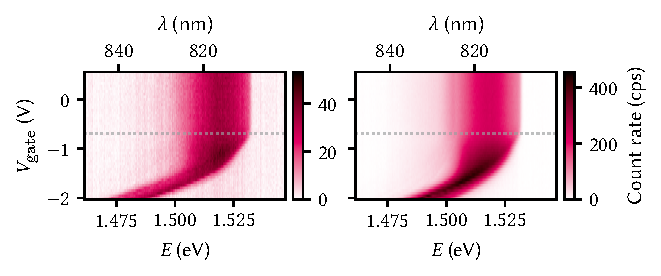
\includegraphics{img/pdf/experiment/honey_H13_stark_shift_vs_gate}
    \caption[
        \sampleid{Honey H13}
        \thewavelength{795},
        \thepower{1}{\micro}.
        \protect\newline
        \imgsource{img/py/experiment/pl.py}
    ]{
        \Gls{pl} as function of gate voltage on a single fan-out gate on the bottom (left) and top (right) side of the membrane.
        The behavior is qualitatively similar but the overall quantum efficiency lower by an order of magnitude for gates on the bottom (as-grown buried) side.
    }
    \label{fig:exp:pl:honey_H13_stark_shift_vs_gate}
\end{figure}

\begin{marginfigure}
    \centering
    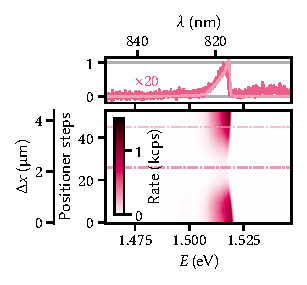
\includegraphics{img/pdf/experiment/fig_F10_positioning}
    \caption[
        \sampleid{Fig F10}
        \thewavelength{795}.
        \protect\newline
        \imgsource{img/py/experiment/pl.py}
    ]{
        \Gls{pl} of the unbiased \gls{qw} as the laser is stepped across a bottom gate.
        The line traces in the upper panel are taken at the positions indicated by dash-dotted lines.
        Positioner steps are converted to distance using a linear fit of the positioner readout after the initial hysteresis has worn off (about \num{10} steps).
        The Fermi edge shows a slight redshift when on top of the gate in this sample.
    }
    \label{fig:exp:pl:fig_F10_positioning}
\end{marginfigure}

\begin{marginfigure}
    \centering
    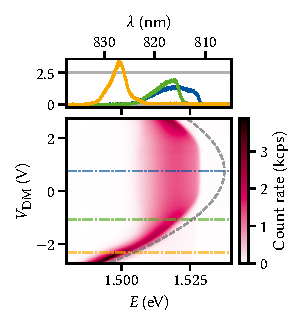
\includegraphics{img/pdf/experiment/doped_M1_05_49-2_difference_mode}
    \caption[
        \sampleid{Doped M1_05_49-2}
        \thevoltage{-1.3}{CM},
        \thewavelength{795}.
        \thepower{10}{\micro}.
        \protect\newline
        \imgsource{img/py/experiment/pl.py}
    ]{
        \Gls{pl} as function of difference-mode voltage on a large exciton trap.
        The observed Stark shift follows roughly the expected quadratic dispersion, but is offset by \qty{0.75}{\volt} with respect to zero bias.
        Dashed gray line is a guide to the eye of a parabola with curvature \qty{-3.5}{\milli\electronvolt\per\volt\squared}.
        Line cuts in the upper panel are taken at the voltages indicated by dash-dotted lines in the lower.
    }
    \label{fig:exp:pl:doped_M1_05_49-2_difference_mode}
\end{marginfigure}

\begin{marginfigure}
    \centering
    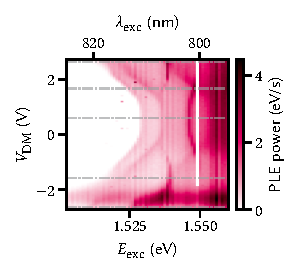
\includegraphics{img/pdf/experiment/doped_M1_05_49-2_ple_margin}
    \caption[
        \sampleid{Doped M1_05_49-2}
        \thevoltage{-1.3}{CM},
        \thepower{1}{\micro}.
        \protect\newline
        \imgsource{img/py/experiment/ple.py}
    ]{
    }
    \label{fig:exp:pl:doped_M1_05_49-2_ple_margin}
\end{marginfigure}

\begin{figure}
    \centering
    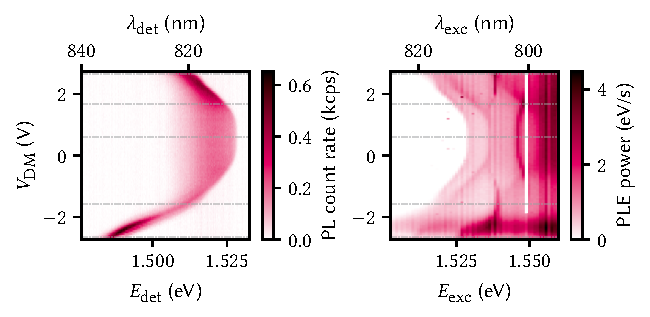
\includegraphics{img/pdf/experiment/doped_M1_05_49-2_ple_wide}
    \caption[
        \sampleid{Doped M1_05_49-2}
        \thevoltage{-1.3}{CM},
        \thepower{1}{\micro}.
        \protect\newline
        \imgsource{img/py/experiment/ple.py}
    ]{
    }
    \label{fig:exp:pl:doped_M1_05_49-2_ple_wide}
\end{figure}

\begin{figure}
    \centering
    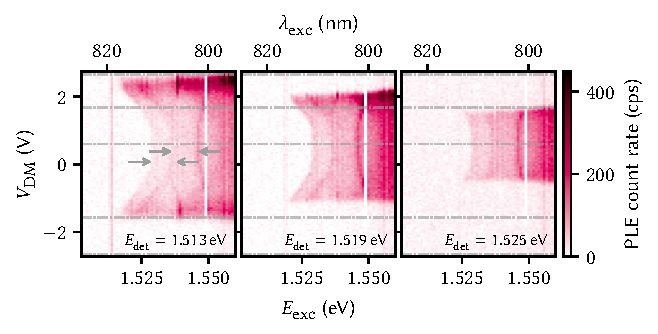
\includegraphics{img/pdf/experiment/doped_M1_05_49-2_ple_delta}
    \caption[
        \sampleid{Doped M1_05_49-2}
        \thevoltage{-1.3}{CM},
        \thepower{1}{\micro}.
        \protect\newline
        \imgsource{img/py/experiment/ple.py}
    ]{
    }
    \label{fig:exp:pl:doped_M1_05_49-2_ple}
\end{figure}

\begin{figure}
    \centering
    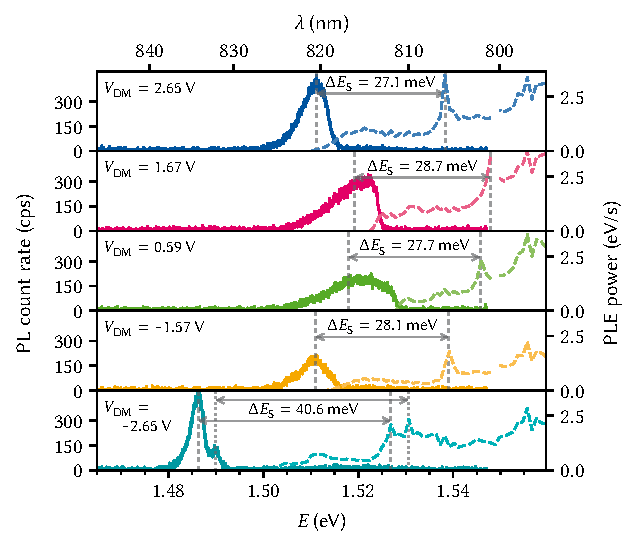
\includegraphics{img/pdf/experiment/doped_M1_05_49-2_ple_cuts}
    \caption[
        \sampleid{Doped M1_05_49-2}
        \thevoltage{-1.3}{CM},
        \thepower{1}{\micro}.
        \protect\newline
        \imgsource{img/py/experiment/ple.py}
    ]{
        \Gls{pl} (solid lines) and \gls{ple} (dashed lines) for different voltages $V_{\mr{DM}}$ (\cf \cref{fig:exp:pl:doped_M1_05_49-2_difference_mode}).
        The \gls{ple} data points correspond to \gls{pl} spectra integrated up to the laser line.
        Arrows indicate the Stokes shift $\Delta E_{\mr{S}}$, which is approximately constant (although assignment of the gap peak is difficult for \qtylist{1.57;0}{\volt}) until the \gls{2deg} is fully depleted and the exciton resonance shifts quadratically with the electric field.
        The features at \qty{1.555}{\electronvolt} do not shift with the voltage and are thus likely unrelated to the trap.
        For the largest voltage, there is another peak at \qty{1.51}{\electronvolt} whose origin is unclear.
    }
    \label{fig:exp:pl:doped_M1_05_49-2_ple_cuts}
\end{figure}

\begin{figure}
    \centering
    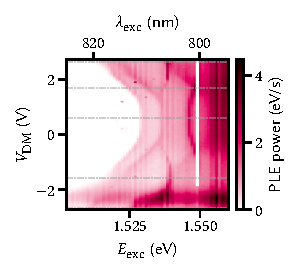
\includegraphics{img/pdf/experiment/doped_M1_05_49-2_ple}
    \caption[
        \sampleid{Doped M1_05_49-2}
        \thevoltage{-1.3}{CM},
        \thepower{1}{\micro}.
        \protect\newline
        \imgsource{img/py/experiment/ple.py}
    ]{
    }
    \label{fig:exp:pl:doped_M1_05_49-2_ple}
\end{figure}

\begin{figure}
    \centering
    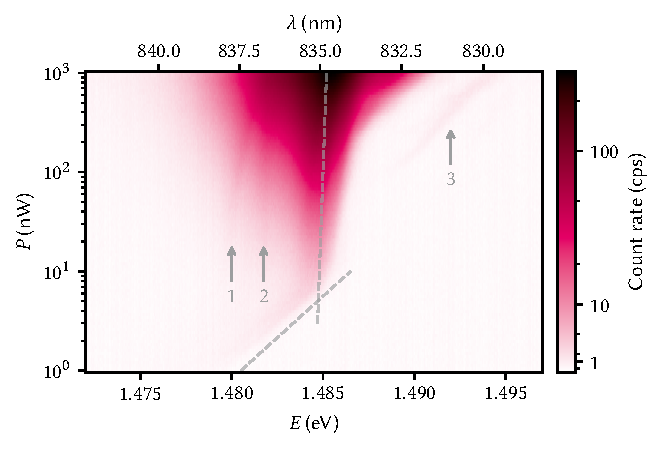
\includegraphics{img/pdf/experiment/doped_M1_05_49-2_power}
    \caption[
        \sampleid{Doped M1_05_49-2}
        \thevoltage{-2.7}{DM},
        \thevoltage{-1.3}{CM},
        \thewavelength{795}.
        \protect\newline
        \imgsource{img/py/experiment/pl.py}
    ]{
        \Gls{pl} as function of excitation power $P$ plotted on a logarithmic color scale.
        Two qualitatively different regimes are indicated by dashed gray lines as guides to the eye; below \qty{10}{\nano\watt}, the main peak displays a blueshift logarithmic in excitation power, $E = \qty{1.485}{\electronvolt} + \qty{5}{\milli\electronvolt}\log_{10} P$.
        Above, the blueshift diminishes significantly.
        Three additional lines, indicated by arrows, with varying power dispersion appear.
    }
    \label{fig:}
\end{figure}

\begin{figure*}
    \centering
    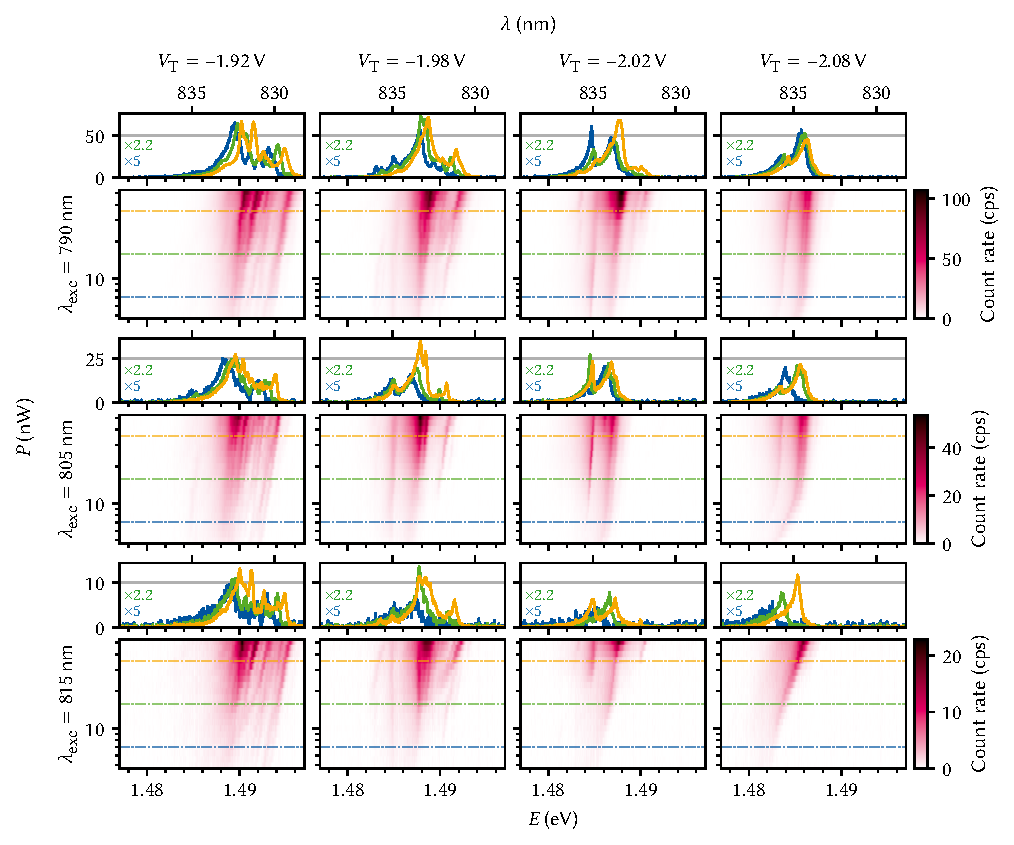
\includegraphics{img/pdf/experiment/doped_M1_05_49-2_multiplets}
    \caption[
        \sampleid{Doped M1_05_49-2}
        \thevoltage{0}{B}.
        \protect\newline
        \imgsource{img/py/experiment/pl.py}
    ]{
        Wide-range \gls{pl} parameter sweep on a large exciton trap plotted as function of excitation power and detection energy.
        Rows are data for three different excitation wavelengths, columns for four different top gate voltages $V_{\mr{T}}$ and share color and line cut scales.
        Line cuts are taken at the indicated positions of $P = \qtylist{7;16;35}{\nano\watt}$ and drawn scaled by the fraction of excitation power with respect to \qty{35}{\nano\watt}.
        % Atomic step fluctuations would shift by ~900 μeV (a = 5.6 Α)
    }
    \label{fig:exp:pl:doped_M1_05_49-2_multiplets}
\end{figure*}

\begin{figure}
    \centering
    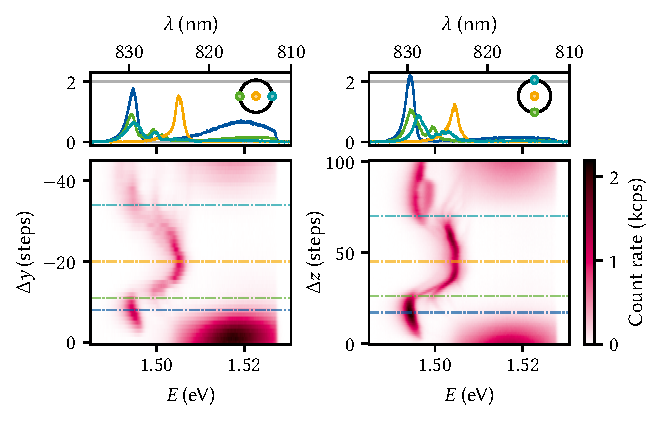
\includegraphics{img/pdf/experiment/doped_M1_05_49-2_positioning}
    \caption[
        \sampleid{Doped M1_05_49-2}
        \thevoltage{-0.43}{DM}
        \thevoltage{-3.75}{CM}
        \thepower{1}{\micro}
        \thewavelength{795}.
        \protect\newline
        \imgsource{img/py/experiment/pl.py}
    ]{
        % z is along gravity
        % y is in plane
    }
    \label{fig:exp:pl:doped_M1_05_49-2_positioning}
\end{figure}